% !TeX root = ../main.tex
\chapter{三维稠密重建}
SLAM全称同时定位与地图构建,在前面我们一直讨论的是定位问题,但这并不表示建图就不重要。一是因为前面的定位、位姿优化等是建图的基础,二是因为人们对建图的要求不同,有的需要简单的稀疏地图,有的需要稠密的地图,大致归纳如下:\par
\begin{enumerate}
	\item 定位:定位是地图的基本功能。在前面的视觉里程计部分,我们讨论了利用局部地图来实现定位;在回环检测部分,我们发现只要有全局描述子信息,机器人的位置信息还能通过回环检测来确定。更进一步,我们还希望地图能够保存下来,分享给其它经过相似场景的机器人,这样我们就能够实现经过一次建模,地图共享。
	\item 导航:导航是指机器人通过视觉或其它传感器信息在地图中进行路径规划,最终到达目的地。稀疏的地图已经不能满足导航的需求,我们需要建立稠密地图。
	\item 避障:避障导航类似需要规划路径避开障碍物,但更注重局部的、动态的障碍物的处理。但仅有稀疏的特征点,我们还很难判断某个特征点是否为障碍物, 所以我们还需要稠密地图。
	\item 重建:重建地图主要用于展示、通讯、增强现实等,这样的地图要求舒服、美观。这种地图也要求是稠密的,而且对它的外观有一些要求,希望能够构建带有纹理的平面。
	\item 交互:交互主要指人与地图之间的互动,这要求机器人对地图有更高层面的认知,这种地图也被称为语义地图。
\end{enumerate}\par
经过前面的SLAM过程,我们已经获得了相机的位置和部分三维特征点的信息,下面就是如何感知周围环境的问题了,这里我们设计实现了一种基于PatchMatch的三维稠密重建方法来进行稠密三维重建。\par
\begin{figure}[H]
	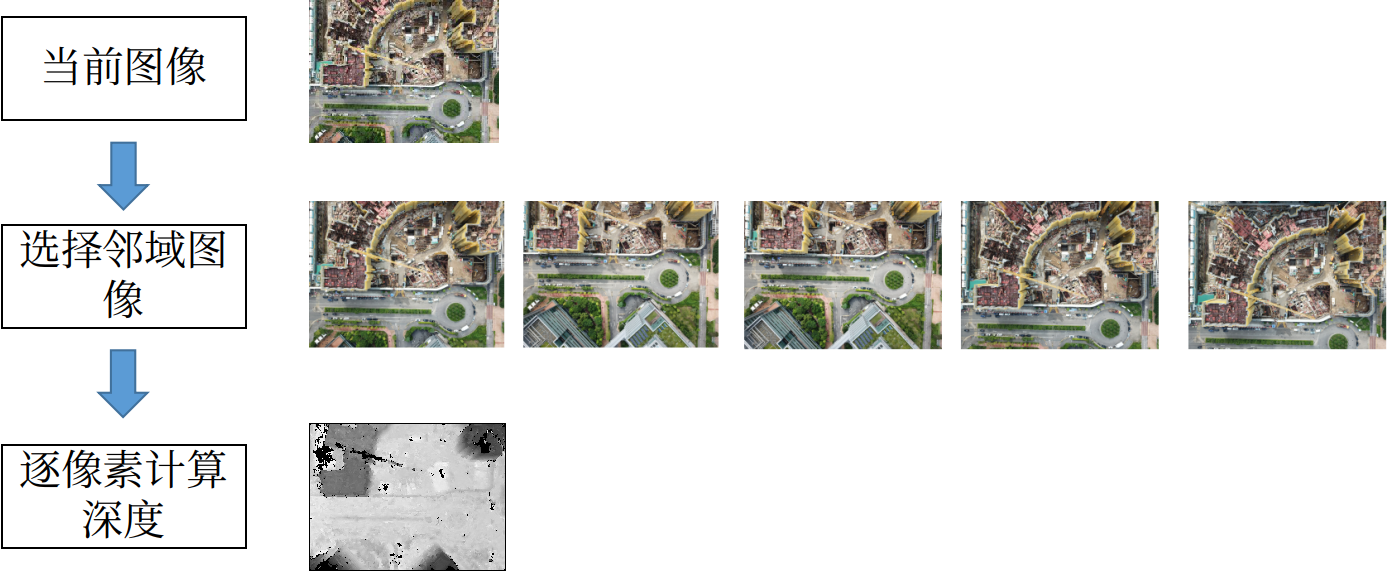
\includegraphics[height=5.5cm]{shenduliucheng}
	\caption{三维重建基本流程}
\end{figure}
PatchMatch的基本思想是假设图像中相邻的像素区域更可能在同一个平面上。这种算法用近乎随机的方法进行全像素计算得到稠密深度图。PatchMatch算法还设计了一个传播的过程,也就是说如果一个点的深度找的很好,那我们可以做出相邻点的深度和平面和该点差不多的假设。那么即便我们随机初始化深度图,只要有一个找到好,这样好的深度就会扩散开,让所有点受益。
\section{邻域图像集合选择}
对于每一张即将计算深度的图像,需要根据邻域图像做立体匹配计算。立体匹配的结果好坏直接影响到重建结果。一张可靠的邻域图像应该跟原图有近似的视角,其次距离也不能相差太多。因此我们考虑这样设计选择算法。
\begin{algorithm}[H]
	\KwResult{N – 邻域图像集合}
	\ForEach{$I_i \in \text{候选邻域图像集合}$}{
		计算$I_i$和$I_{cur}$的共视特征点CorPoints \;
		\ForEach{$Point_k \in CorPoints$}{
			计算Point与相机光心夹角$\theta_{i}^{k}$\;
			\If{$\theta_{i}^{k}<\frac{\pi}{3}$}{
				$Score_i$+=1\;
			}
		}
	}
	将$Score_i$降序排列,取前8个作为邻域图像集N\;
	\caption{邻域选取算法}
	\label{algo:pickneighber}
\end{algorithm}
\section{深度图计算}
深度图计算主要分为三个过程:深度范围估计,随机初始化,传播更新深度。
\subsection{深度范围估计}
对于每张图,我们需要指定一个初始的深度范围。这个范围可以通过图像对应的特征点的深度来初步估计。对于任意该图像可见的三维点来说,已知图像的$R,t$我们可以将其变换到当前相机坐标系下:
\begin{equation}
	P_c = \boldsymbol{R}P_w+t
\end{equation}
其中$P_c$的第三维表示深度。我们可以统计该图像所能观察到所有的三维点在该相机坐标系下的深度值,并从大到小排序,那么我们可以认为图像的深度范围在$(d_{min},d_{max})$之间。
\subsection{随机初始化}
我们再更详细的描述一下PatchMatch的思想:对于当前图像和邻域图像集合中的任一图像,对于当前图像的每一个像素,都会有这样一个平面——该像素以及像素周围的像素块(Patch)经过该平面利用单应矩阵投影至邻域图像上的时候,该像素块和邻域图像上的像素块是相似的。\par
那么基于这样的思想,我们随机初始化就是去初始化每个像素对应的平面。\par
\begin{figure}[H]
		\centering
		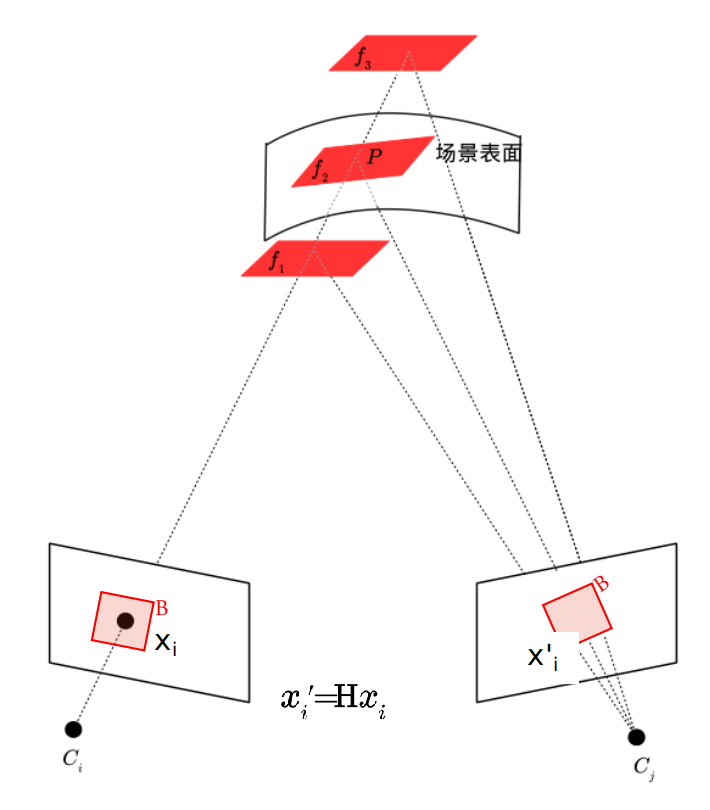
\includegraphics[height=7cm]{randomplane}
		\caption{单应平面}
		\label{randomplane}
\end{figure}
如图\ref{randomplane}所示,我们随机初始化三个平面:$f_1,f_2,f_3$,可以看到$f_2$是估计的最好的平面。我们目测很容易就能看出来$f_2$是最优平面,但实际计算的时候我们是不知道真实平面的。这个时候就要通过归一化互相关匹配(NCC)算法来对两个像素块进行匹配程度计算:
\begin{equation}
	NCC(i,j)=\frac{\sum_{i=m}^{m / 2} \sum_{2 j=n}^{n / 2} f(x+i, y+j) \cdot t(i, j)-m \cdot n \cdot \mu_{f} \cdot \mu_{t}}{\left\{\left(\sum_{i} \sum_{j} f^{2}(x+i, y+j)-m \cdot n \cdot \mu_{f}^{2}\right)\left(\sum_{t} \sum_{j} r^{2}(x+i, y+j)-m \cdot n \cdot \mu_{r}^{2}\right)\right\}^{\frac{1}{2}}}
\end{equation}
其中:
\begin{equation}
\begin{array}{l}{\mu_{f}(x, y)=\frac{1}{m \cdot n} \sum_{i=m}^{m / 2} \sum_{j=-n}^{n / 2} f(x+i, y+j)} \\ {\mu_{t}(x, y)=\frac{1}{m \cdot n} \sum_{i=-m}^{m / 2} \sum_{j=n}^{n / 2} t(i, j)}\end{array}
\end{equation}
所谓归一化互相关,实际上就是将3$\times$3的Patch拉成1$\times$9的向量,并且归一化其模为1。然后将左右两图的向量点乘,结果越接近1越相似。\par
那么对于原图像上的像素$x_i$,我们会随机估计50个不同深度,不同朝向的平面,对于每个平面我们都用单应矩阵求解出投影到$x^{\prime}_i$处的Patch,再用NCC方法计算该平面的得分。取出最优的平面作为该点的初始化平面。
\begin{algorithm}[H]
	\KwResult{\\$score_{best}$ – 随机初始化平面得分\\
	$nghbr_{best}$ – 最高得分对应的邻域图像ID} 
	\ForEach{$p_i \in I_{cur} $}{
		$score^i_{best}=-1;nghbr^i_{best}=0$\;
		\ForEach{$I_{nghbr} \in N$}{
			\If{当前得分$scoreI_{nghbr}>score_{best}$}
			{$score_{best}=scoreI_{nghbr}$\\
			$ngbr_{best}=I_{nghbr}$}	
		}
	}
	\caption{随机初始化算法}
	\label{algo:rabdom}
\end{algorithm}
\subsection{传播更新深度}
初始化深度后,当前图像上$I {cur}$ 中的每个像素都分配了一个空间平面作为其单应平面。但这个是初步的结果,我们需要对这些平面进行修正。先从左上向右下按行顺序传播更新深度,然后从右下向左上再按行顺序传播一次更新深度,通过不断迭代这两步,更新深度图,本文迭代数是3。
\begin{algorithm}[H]
	\KwData{\\$d_{i,j}$:像素点$(i,j)$的深度\\
	$M(i,j)$是像素点$(i,j)$的邻近像素点集合\\
	Iteration 迭代次数本文设为3}
	\ForEach{$d_{i,j}\in depth_{cur}$}{
		\If{$d_{i,j}\neq 0$}{
			\For{$(i_{adj},j_{adj}) \in M(i,j)$}{
				\If{$d_{i_{adj},j_{adj}}\neq 0$}
				{对于像素点$(i,j)$,计算$(i_{adj},j_{adj})$对应世界平面时的相似度得分 \; 
				\If{当前得分$score >score_{(i,j)}$}{
				反投影得到像素点$(i,j)$的深度并更新对应的$depth,plane,score,nghbr$\;}}
			}
		}
		\For {$k<$Iteration}{
		对当前对应的最优深度和最优平面法向量分别加服从均匀分布的扰动,求得分 \;
		\If {当前相似度得分$score >score_{(i,j)}$}{
			反投影得到像素点$(i,j)$的深度并更新对应的$depth,plane,score,nghbr$;}
		$depthRange *= 0.5,normalRange *= 0.5;$
		}
	求当前最优平面和随机的其他一个邻近图像的相似度得分 \; 
		\If{当前得分$score >score_{(i,j)}$}	 
 		{反投影得到像素点$(i,j)$的深度并更新对应的$depth,plane,score,nghbr$ \;}
	}
	\caption{方向传播更新深度算法} 
	\label{PatchMatchUpdatePixel_alg} 
\end{algorithm}
如算法\ref{PatchMatchUpdatePixel_alg}, 更新深度分为三个步骤:\par
首先,遍历图像中每个像素点,每个像素点都先和它左边和上面的像素进行对比。如果左边和上边的深度不为0,那么就分别以他们的平面为单应平面进行投影并计算score。如果计算得到的score比自身的socre好,就将该像素的平面更新为较好的平面。\par
然后再对这个新平面进行微调,看附近是否有更好的更合适的平面。若有则再次更新平面。这样就实现了一次从左上到右下的传播。\par
最后同样的从右下到左上再传播一次,操作相同。
\section{实验结果}
该基于PatchMatch的稠密重建方法用 C++ 编程语言实现,在数据集上进行了测试,面对普通场景基本能取得不错的结果。但是面对复杂情况比如树和楼混合在一起的时候比较难以分辨。\par
实验采用的计算机配置是:Intel(R) Core(TM) i7-4720HQ CPU@2.6GHz,8G 内存,在 64 位 Deepin操作系统下运行。
\begin{figure}
	\centering
	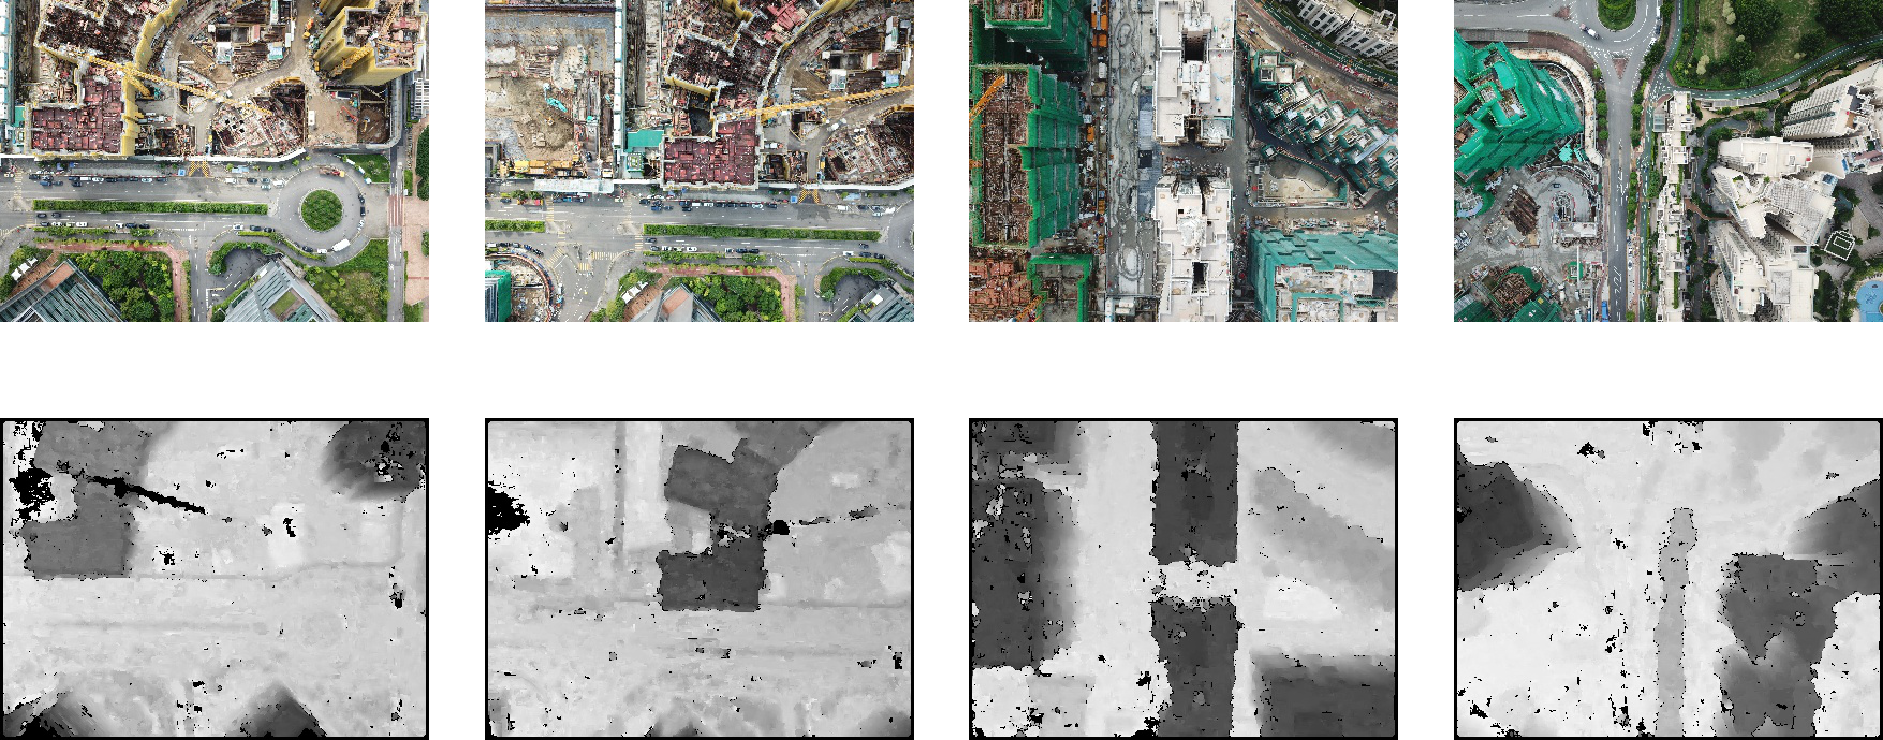
\includegraphics[height=5cm]{shendu}
	\caption{单张深度信息}
\end{figure}

\begin{figure}[H]
	\centering
	\begin{subfigure}[ht]{0.4\textwidth}
		\centering
		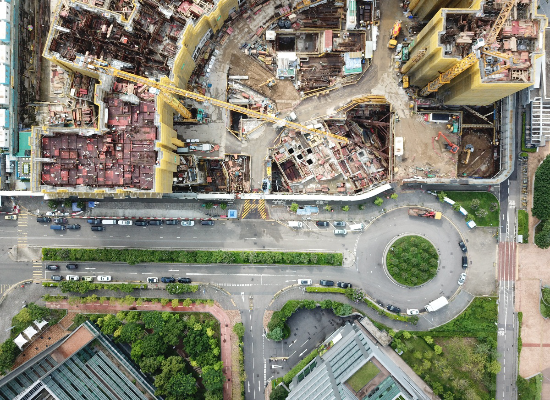
\includegraphics[height=4cm]{fig1_1}
	\end{subfigure}
	\quad
	\begin{subfigure}[ht]{0.4\textwidth}
		\centering
		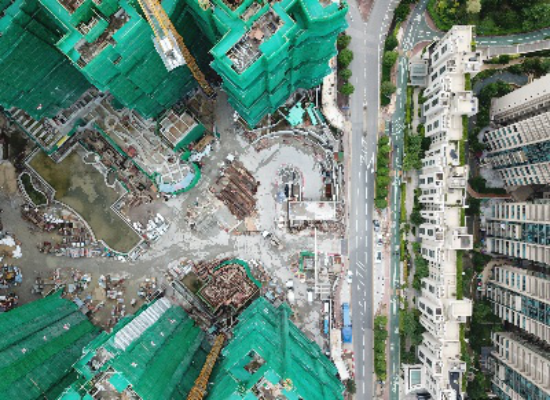
\includegraphics[height=4cm]{fig2_1}
	\end{subfigure}\\
	\begin{subfigure}[ht]{0.4\textwidth}
		\centering
		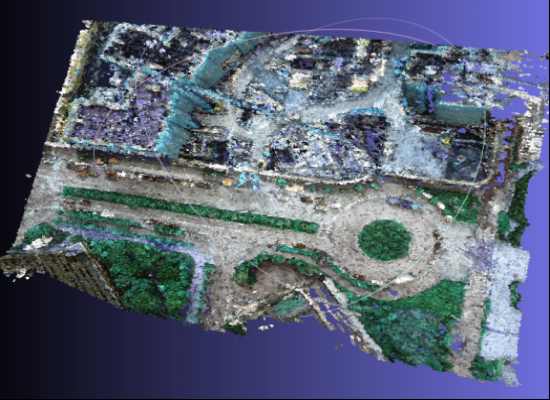
\includegraphics[height=4cm]{re1_1}
	\end{subfigure}
	\quad
	\begin{subfigure}[ht]{0.4\textwidth}
		\centering
		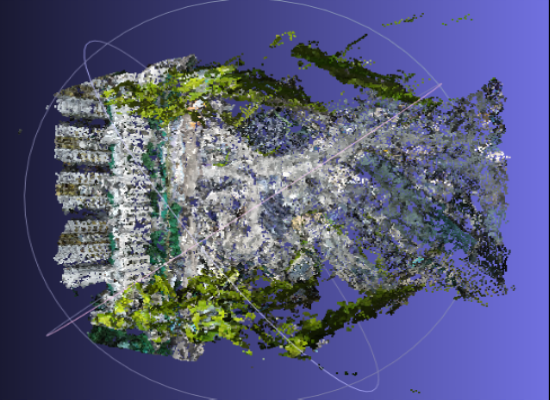
\includegraphics[height=4cm]{re2_1}
	\end{subfigure}
\begin{subfigure}[ht]{0.4\textwidth}
	\centering
	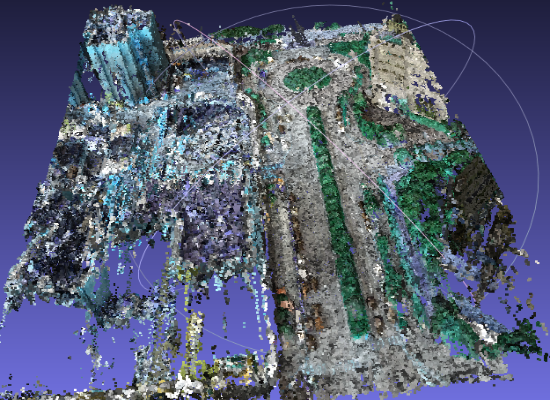
\includegraphics[height=4cm]{re1_2}
	\subcaption{场景a}
\end{subfigure}
\quad
\begin{subfigure}[ht]{0.4\textwidth}
	\centering
	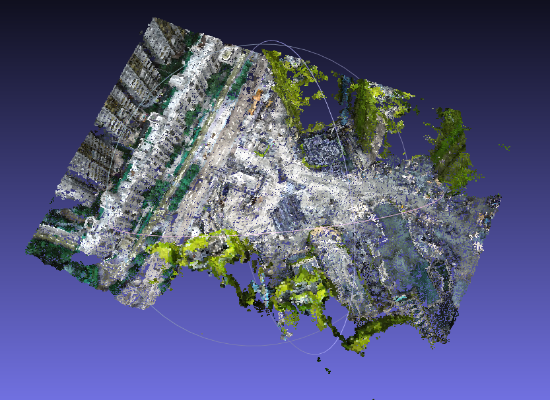
\includegraphics[height=4cm]{re2_2}
	\subcaption{场景b}
\end{subfigure}
	\caption{PatchMatch稠密重建}
\end{figure}
根据基于PatchMatch的稠密点云重建结果来看,我们通过SLAM提供的相机位姿还是比较准确的。重建结果中平面基本仍旧是平面,一些关键的边缘部分识别情况尚可。但是目前做的PatchMatch只计算了一张图上的像素点,并没有多帧计算相互校验,因此重建结果在边缘部分并不好。之后多帧同时重建效果会更好。\par
在本机用Svar库统计时间结果如下表:
\begin{table}[H]
	\centering
	\begin{tabular}{cccccc}
		\toprule
		FUNCTION             & CALLS & MIN.T   & MEAN.T  & MAX.T   & TOTAL   \\ \midrule
		RandomInitialization & 1     & 137.2ms & 137.2ms & 137.2ms & 137.2ms \\ \hline
		ComputeIgnoreMask    & 1     & 16.6ms  & 16.6ms  & 16.6ms  & 16.6ms  \\ \hline
		PatchMatchIter       & 3     & 2.5 s   & 2.5 s   & 2.6 s   & 7.6 s   \\ \hline
		computeDepth         & 1     & 7.8 s   & 7.8 s   & 7.8 s   & 7.8 s   \\ \hline
		computeMaxMindepth   & 896   & 111.0ns & 164.4ns & 1.0us   & 147.3us \\ \hline
		Total                & 1     &         &         &         & 10.3 s  \\ \bottomrule
	\end{tabular}
\end{table}\par
在选用8张图为辅助计算的时候,全像素计算一张图的深度信息大概需要8秒左右。这个速度相比于目前市面上常见的软件来说表现平平。但是仍然有加速的空间。\par
一方面由于PatchMatch的BrutalForce计算方法跟相邻像素的深度值无关,因此我们可以考虑利用GPU并行计算的特性来对这个计算过程进行加速,让全像素同时进行计算。另一方面我们发现,在实际的三维重建贴图过程中,有用的只是图片的边缘部分,因此我们考虑仅求解图像的轮廓。从全像素求解到仅求解轮廓部分,会让计算像素的数量级大大下降,从而提高了速度。这样下来计算性能应该能提升到每秒数十帧到上百帧的层次。




